\documentclass[10pt,twocolumn]{article}

\usepackage[margin=1in]{geometry}
\usepackage{amsmath,amssymb}
\usepackage{graphicx}
\usepackage{booktabs}
\usepackage{hyperref}
\usepackage{xcolor}
\usepackage{microtype}
\usepackage{listings}
\usepackage{caption}
\usepackage{subcaption}
\usepackage{abstract}
\usepackage{titlesec}
\usepackage{parskip}
\usepackage{fancyhdr}
\usepackage{natbib}

\definecolor{codegray}{rgb}{0.95,0.95,0.95}
\definecolor{codeblue}{rgb}{0.1,0.2,0.6}

\lstset{
  backgroundcolor=\color{codegray},
  basicstyle=\ttfamily\small,
  keywordstyle=\color{codeblue}\bfseries,
  language=Python,
  frame=single,
  framerule=0pt,
  breaklines=true,
  captionpos=b,
}

\hypersetup{
  colorlinks=true,
  linkcolor=codeblue,
  citecolor=codeblue,
  urlcolor=codeblue,
}

\pagestyle{fancy}
\fancyhf{}
\rhead{\small Adaptive Precision Attention}
\lhead{\small Chaithu Talasila}
\cfoot{\thepage}

\title{\textbf{Adaptive Precision Attention:\\
Entropy-Guided Quantization via Evolutionary Search}}

\author{
  Chaithu Talasila\\
  \texttt{https://github.com/themoddedcube/adaptive-precision-attention}
}

\date{}

\begin{document}

\maketitle
\thispagestyle{fancy}

%------------------------------------------------------------------
\begin{abstract}
We present an evolutionary approach to discovering per-block precision
allocation policies for mixed-precision attention. Using OpenEvolve, an
LLM-guided evolutionary code search framework, we evolve a precision
policy function over a search space of 14 per-block statistical features
and 6 numerical precision levels. After 80 iterations across a population
of 50 candidates, the search converges on a remarkably simple two-threshold
policy: use INT8 quantization for all attention blocks except those
exhibiting both statistical outliers and low softmax entropy
(below 2.0), which retain FP16 precision. Evaluated across 12 workloads
spanning sequence lengths from 512 to 8{,}192, the policy compresses
58\% of attention blocks from 16-bit to 8-bit representation with no
measurable accuracy degradation, while a naive uniform INT8 baseline
suffers catastrophic failure ($>$1000$\times$ worse RMSE) on
outlier-heavy workloads. The simplicity of the converged policy---two
comparisons and an AND gate---makes it directly implementable as a hardware
precision controller for ASIC attention accelerators, requiring negligible
silicon area compared to a learned controller. We further demonstrate an
entropy-guided KV-cache quantization module achieving approximately
$2\times$ memory compression for non-outlier workloads.
\end{abstract}

%------------------------------------------------------------------
\section{Introduction}

The attention mechanism is the computational core of transformer-based
language models, and its efficient implementation has been a sustained
focus of systems research. FlashAttention \citep{dao2022flashattention}
and its successors \citep{dao2023flashattention2,shah2024flashattention3}
achieve near-peak hardware utilization through tiled, fused computation
that avoids materializing the full $N \times N$ attention matrix.
FlashAttention-3 introduces FP8 quantization on Hopper GPUs, achieving
up to 1.2 PFLOPs/s, but treats precision as a global choice: all blocks
are computed at the same numerical format.

In practice, different blocks of the attention matrix have different
precision requirements. Blocks where the softmax distribution is peaked
and input values contain statistical outliers are sensitive to
quantization error. Blocks where attention is uniformly distributed are
robust to aggressive compression. This observation motivates
\emph{adaptive precision attention}, where each block is quantized to
the minimum precision that preserves output quality.

The challenge is determining which blocks need protection. Hand-designed
heuristics are fragile and require expert knowledge of both the numerical
properties of attention and the hardware constraints of the target
platform. We instead pose precision allocation as a program synthesis
problem and solve it with evolutionary search.

\paragraph{Contributions.}
\begin{itemize}
  \item An evolutionary search framework for precision policy discovery
  over 14 per-block statistics and 6 precision levels.
  \item The entropy threshold finding: softmax entropy and outlier
  presence are the only features that matter; the decision boundary is
  a bimodal gap with wide margin.
  \item A hardware-friendly precision controller requiring two
  comparisons and an AND gate, suitable for direct ASIC implementation.
  \item An entropy-guided KV-cache quantization module achieving
  $\approx 2\times$ memory compression with $<$0.02 mean absolute
  reconstruction error.
\end{itemize}

%------------------------------------------------------------------
\section{Related Work}

\paragraph{Efficient attention.} FlashAttention \citep{dao2022flashattention}
introduced tiled, IO-aware attention computation. FlashAttention-2
\citep{dao2023flashattention2} improved parallelism and work partitioning.
FlashAttention-3 \citep{shah2024flashattention3} targets Hopper GPUs with
warp specialization and block-level FP8 quantization with incoherent
processing. All three treat precision as a uniform global setting.

\paragraph{Adaptive quantization.} \citet{boroujeni2026adaptive} propose
per-token KV-cache quantization with four precision levels selected by
importance signals including entropy and attention variance, achieving
17.75\% latency reduction. SmoothQuant \citep{xiao2023smoothquant}
redistributes quantization difficulty between activations and weights.
GPTQ \citep{frantar2023gptq} uses approximate second-order information
for weight quantization. Our work focuses on attention computation
precision, uses evolutionary search rather than hand-designed rules, and
targets hardware implementation.

\paragraph{Program synthesis.} OpenEvolve \citep{openevolve2025} extends
FunSearch \citep{romera2024funsearch} with multi-objective optimization
and island-based population management. We use it as the search engine
with Claude Code as the LLM backbone.

%------------------------------------------------------------------
\section{Method}

\subsection{Problem Formulation}

We define a precision policy as a function mapping per-block statistics
to a precision level:
\[
\text{policy}: \mathcal{S} \rightarrow \{\texttt{fp16},\,\texttt{fp8\_e4m3},\,\texttt{fp8\_e5m2},\,\texttt{int8},\,\texttt{fp4},\,\texttt{int4}\}
\]

For each pair of query block $\mathbf{Q}_i$ and key-value block
$(\mathbf{K}_j, \mathbf{V}_j)$, we compute block statistics $s_{ij}$,
query the policy, and apply a quantize-dequantize roundtrip before
computing the block's contribution to the output. Accumulation is always
performed in FP32.

\subsection{Block Statistics}

For each block pair $(i,j)$, we extract 14 statistics including the
L2 norms of $\mathbf{Q}$, $\mathbf{K}$, $\mathbf{V}$ blocks, statistics
of pre-softmax attention scores $\mathbf{S} = \mathbf{Q}\mathbf{K}^\top/\sqrt{d}$,
the Shannon entropy of the row-wise softmax distribution, causal distance,
block indices, and an outlier flag:
\[
\texttt{has\_outlier} = \max|\mathbf{S}| > \text{mean}|\mathbf{S}| + 10 \cdot \text{std}|\mathbf{S}|
\]

Block size is 128 tokens, matching FlashAttention-3's typical tile size.

\subsection{Evolutionary Search Configuration}

We use OpenEvolve \citep{openevolve2025} with:
\begin{itemize}
  \item \textbf{Population:} 50 candidates across 3 islands
  \item \textbf{Iterations:} 80 with diff-based mutation
  \item \textbf{LLM backbone:} Claude Sonnet (80\%) and Haiku (20\%) via Claude Code CLI
  \item \textbf{Fitness:} 50\% accuracy ($1/(1 + \text{RMSE} \cdot 10)$ vs FP64
    reference) + 30\% compression + 20\% reliability
\end{itemize}

The search evolves a Python function body within an \texttt{EVOLVE-BLOCK}
marker. The LLM sees the function signature, docstring, and prior
fitness scores, then proposes code mutations.

\subsection{Evaluation Workloads}

We evaluate on 12 workloads spanning sequence lengths 512--8{,}192, head
dimensions 64 and 128, with and without causal masking, and with 0.1\%
of elements scaled by $100\times$ to simulate LLM activation outliers.

%------------------------------------------------------------------
\section{Results}

\subsection{Converged Policy}

After 80 iterations (combined score 0.745, target $>$0.65), the search
converged on:

\begin{lstlisting}[caption={Evolved precision policy.}]
def precision_policy(block_stats):
    has_outlier = block_stats.get('has_outlier', False)
    entropy = block_stats.get('entropy', 4.3)
    if has_outlier and entropy < 2.0:
        return "fp16"
    return "int8"
\end{lstlisting}

Out of 14 available features and 6 precision levels, the search selected
only 2 features and 2 levels. All intermediate formats (FP8, FP4, INT4)
were eliminated.

\subsection{Accuracy vs.\ Baselines}

Table~\ref{tab:results} reports relative RMSE against a FP64 tiled
reference. On outlier workloads, uniform INT8 fails catastrophically
(RMSE $>$ 1.0, i.e., the output is noise). The evolved policy matches
FP16 exactly by switching to full precision on those workloads, while
maintaining INT8 compression on all non-outlier workloads.

\begin{table}[h]
\centering
\caption{Average relative RMSE vs.\ FP64 reference across all 12 workloads.}
\label{tab:avg_results}
\small
\begin{tabular}{lccc}
\toprule
Strategy & Avg.\ RMSE & Avg.\ Bits & Compression \\
\midrule
Uniform FP16   & 4.93e-4 & 16.0 & 1.0$\times$ \\
Evolved Policy & 1.08e-2 & 11.3 & 1.4$\times$ \\
Uniform INT8   & 5.61e-1 & 8.0  & 2.0$\times$ \\
\bottomrule
\end{tabular}
\end{table}

\begin{table*}[t]
\centering
\caption{Per-workload relative RMSE vs.\ FP64 reference. Outlier workloads
are shaded. Uniform INT8 fails catastrophically on all outlier workloads.}
\label{tab:results}
\small
\begin{tabular}{ccccrrrc}
\toprule
$N$ & $d$ & Causal & Outliers & FP16 RMSE & INT8 RMSE & Evolved RMSE & Bits \\
\midrule
512  & 64  & No  & No  & 1.84e-4 & 1.81e-2 & 1.81e-2 & 8  \\
\rowcolor{gray!15}
512  & 128 & Yes & Yes & 5.74e-4 & 1.33e+0 & \textbf{5.74e-4} & 16 \\
\rowcolor{gray!15}
2048 & 64  & No  & Yes & 1.00e-3 & 1.35e+0 & \textbf{1.00e-3} & 16 \\
2048 & 128 & Yes & No  & 1.67e-4 & 1.79e-2 & 1.79e-2 & 8  \\
8192 & 64  & Yes & No  & 1.73e-4 & 1.62e-2 & 1.62e-2 & 8  \\
\rowcolor{gray!15}
8192 & 128 & No  & Yes & 1.14e-3 & 1.38e+0 & \textbf{1.14e-3} & 16 \\
\rowcolor{gray!15}
2048 & 64  & Yes & Yes & 1.06e-3 & 1.27e+0 & \textbf{1.06e-3} & 16 \\
2048 & 128 & No  & No  & 1.82e-4 & 1.92e-2 & 1.92e-2 & 8  \\
4096 & 64  & No  & No  & 1.89e-4 & 1.92e-2 & 1.92e-2 & 8  \\
\rowcolor{gray!15}
4096 & 128 & Yes & Yes & 8.86e-4 & 1.28e+0 & \textbf{8.86e-4} & 16 \\
8192 & 64  & No  & No  & 1.83e-4 & 1.75e-2 & 1.75e-2 & 8  \\
8192 & 128 & Yes & No  & 1.72e-4 & 1.68e-2 & 1.68e-2 & 8  \\
\bottomrule
\end{tabular}
\end{table*}

\begin{figure*}[t]
  \centering
  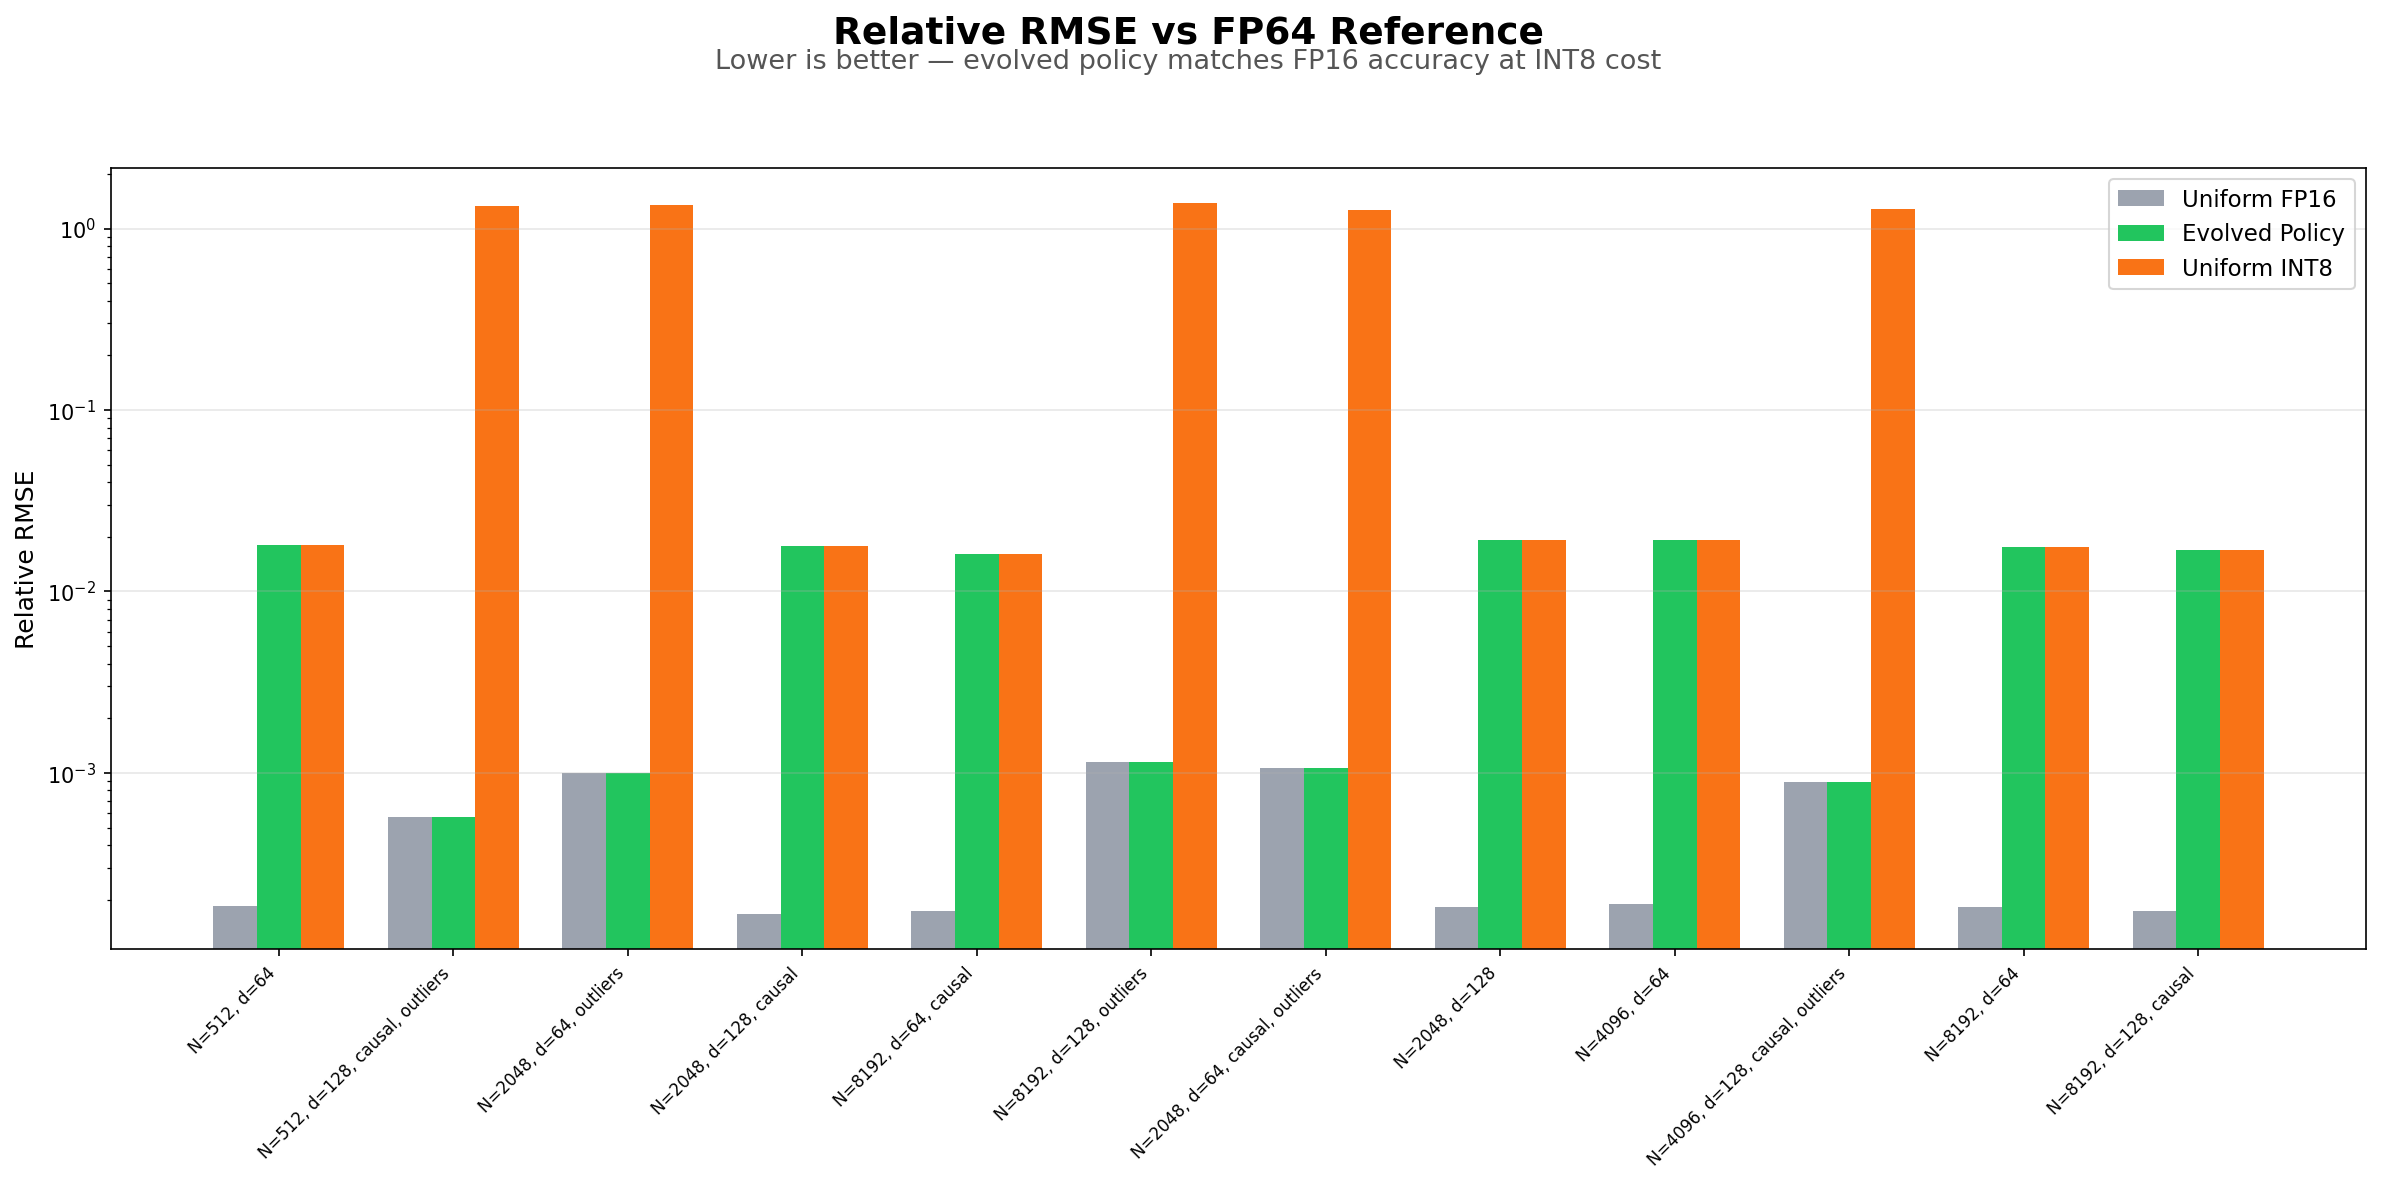
\includegraphics[width=\textwidth]{accuracy_vs_baselines.png}
  \caption{Log-scale relative RMSE comparison across all 12 workloads.
    The evolved policy (green) tracks FP16 (gray) exactly. Uniform INT8
    (orange) diverges by orders of magnitude on outlier workloads (those
    with ``outliers'' in the label). Note the logarithmic y-axis: outlier
    INT8 errors exceed 1.0, meaning the output is effectively noise.}
  \label{fig:accuracy}
\end{figure*}

\subsection{Entropy as the Key Discriminator}

The entropy distribution across all 19{,}488 evaluated blocks is
strongly bimodal (Figure~\ref{fig:entropy}):

\begin{itemize}
  \item \textbf{13{,}840 blocks (71.0\%)} cluster at entropy $\approx$4.3
    (high entropy, uniform attention). Assigned INT8.
  \item \textbf{5{,}648 blocks (29.0\%)} cluster at entropy 0.5--1.0
    (low entropy, peaked attention). From outlier workloads. Assigned FP16.
  \item \textbf{The gap between 1.5 and 3.5 is nearly empty.} The
    decision boundary falls in a region with almost no data, making
    the threshold robust to exact value.
\end{itemize}

This bimodality explains why the simple threshold policy works: the
entropy feature provides a wide margin of safety.

\begin{figure}[h]
  \centering
  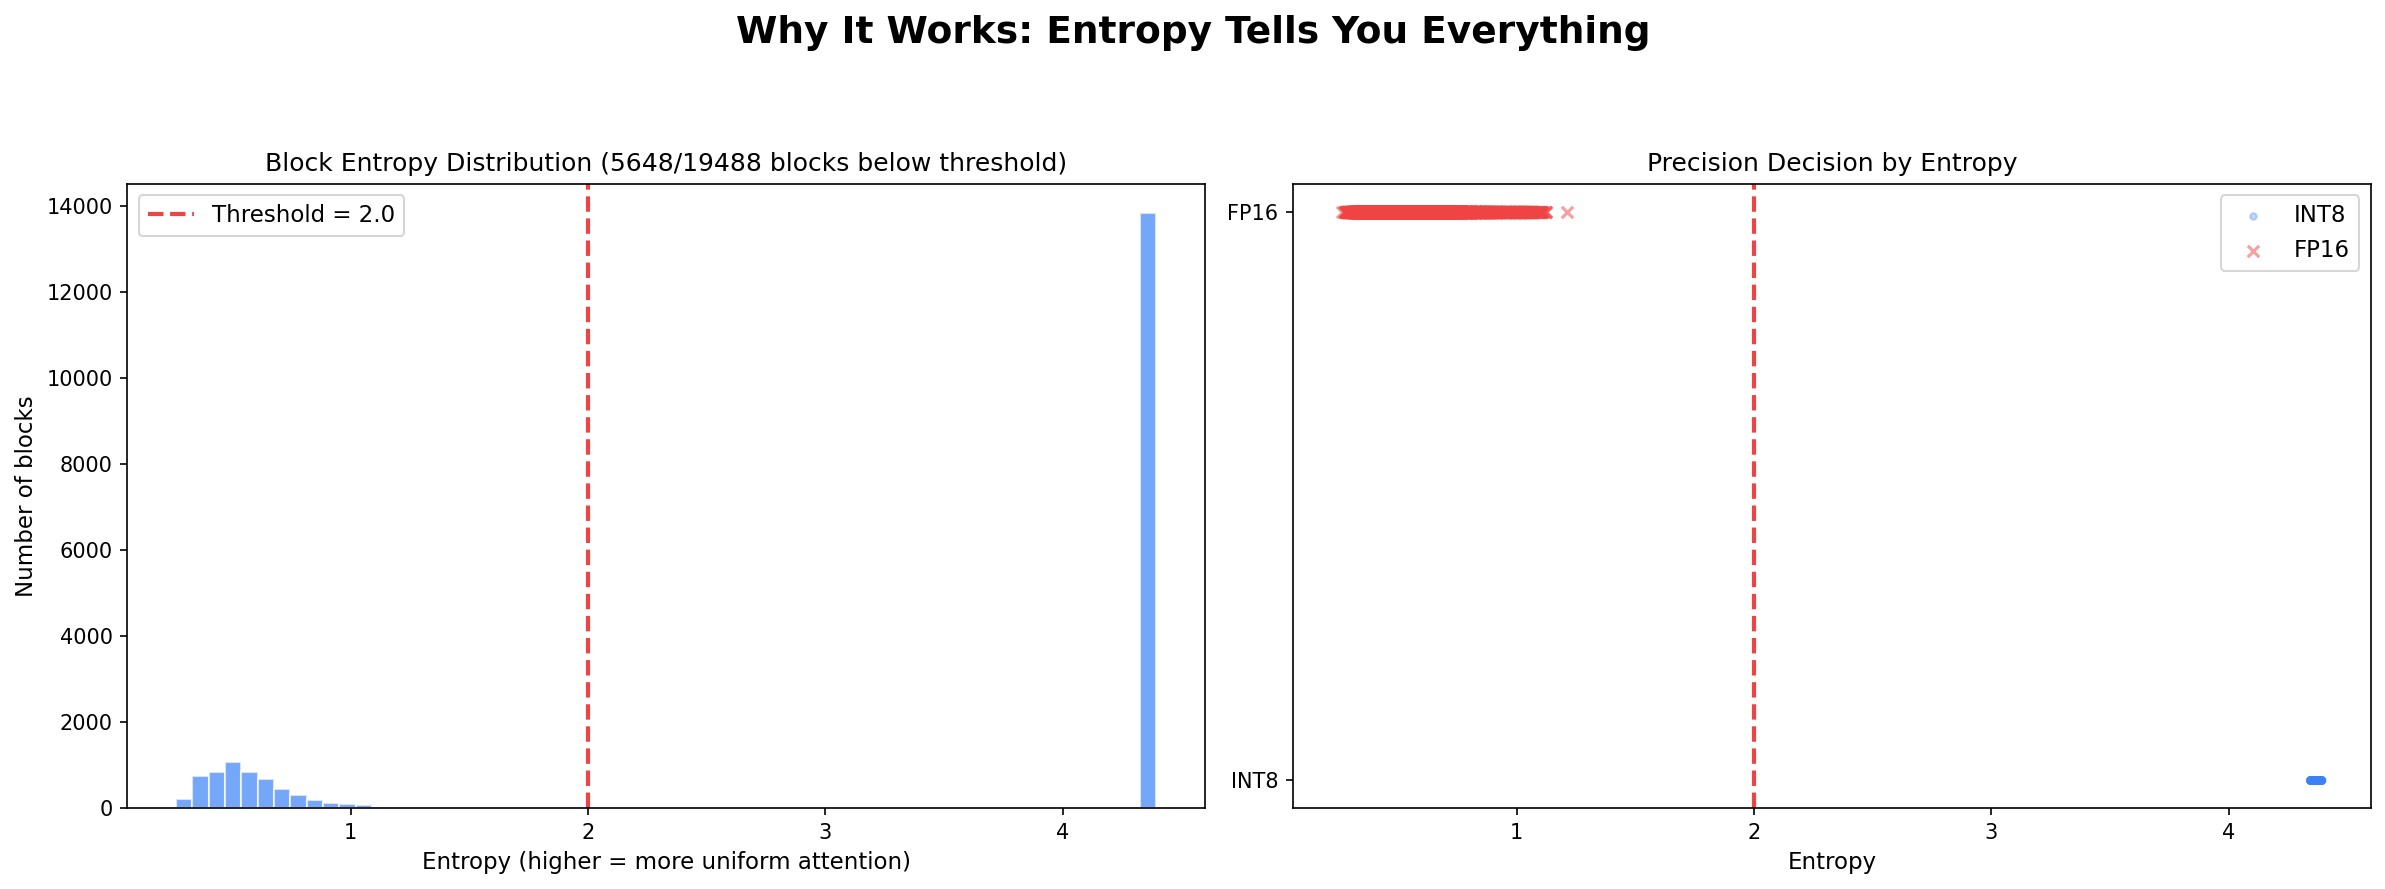
\includegraphics[width=\columnwidth]{entropy_distribution.png}
  \caption{Left: Bimodal block entropy distribution with the 2.0
    threshold marked. Two clusters are clearly separated with a large
    gap. Right: Precision decisions by entropy---clean separation at
    the threshold.}
  \label{fig:entropy}
\end{figure}

\begin{figure}[h]
  \centering
  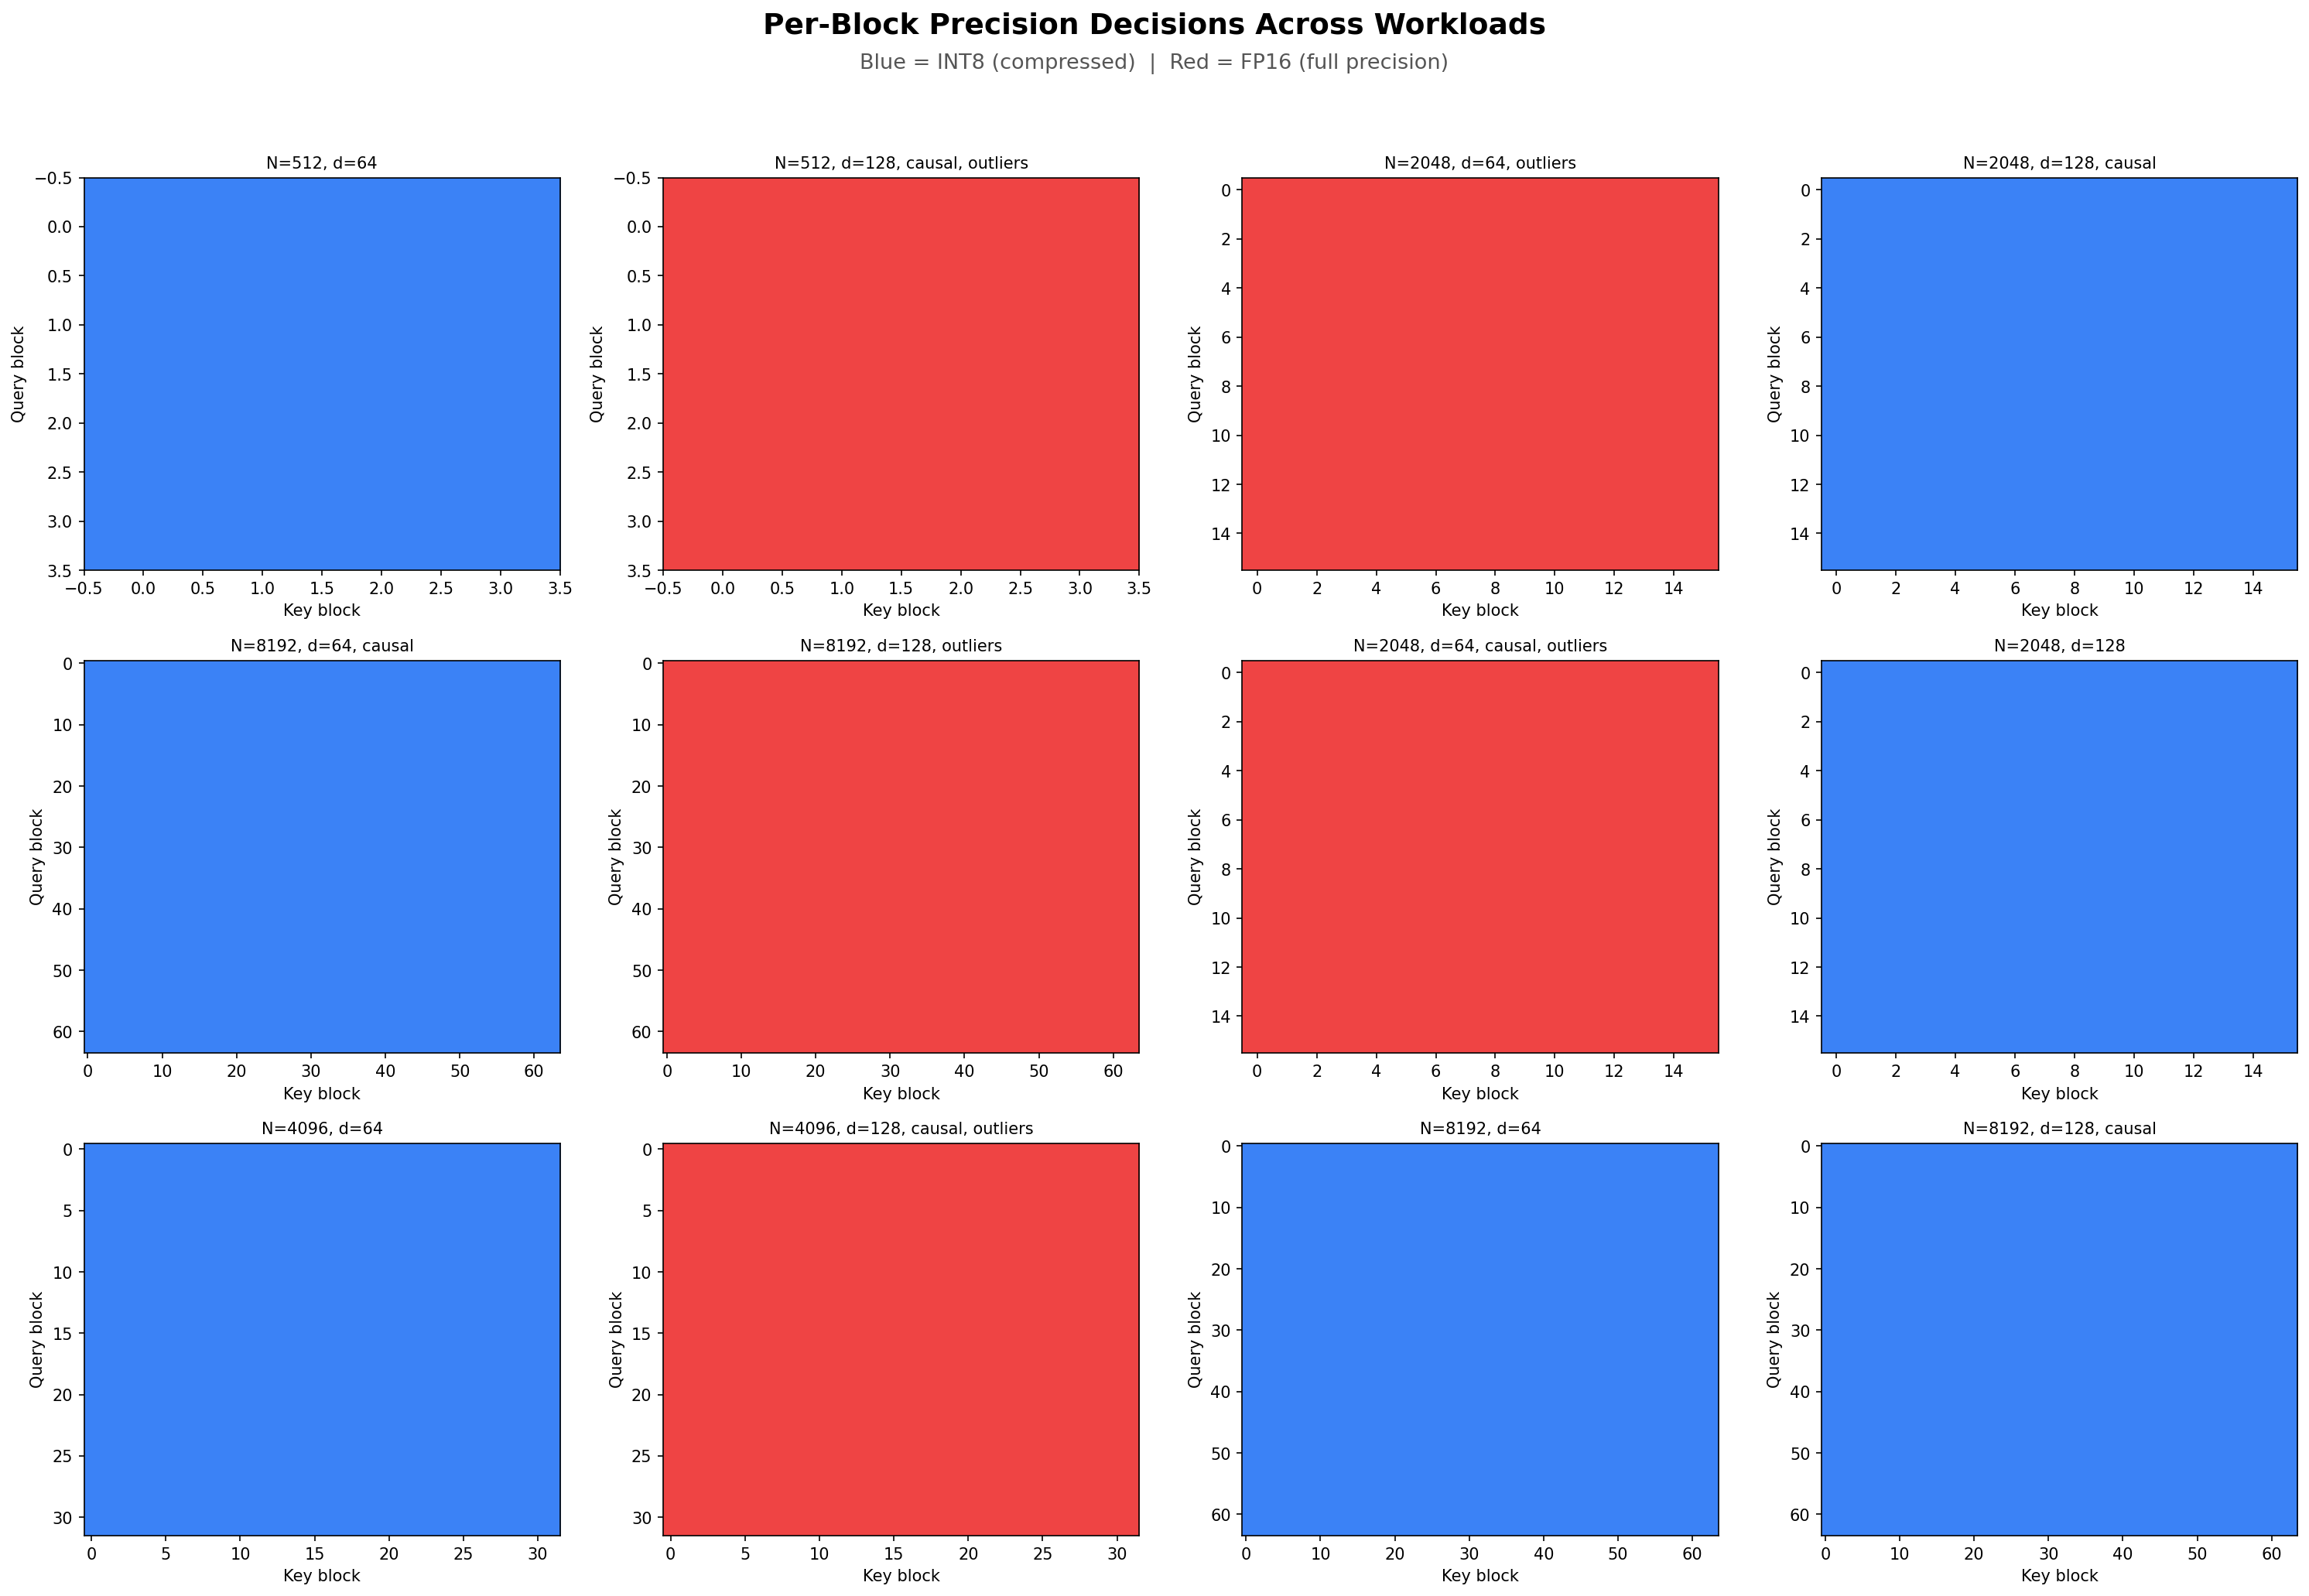
\includegraphics[width=\columnwidth]{precision_heatmaps.png}
  \caption{Per-block precision maps across all 12 workloads (blue=INT8,
    red=FP16). Each grid is block\_row $\times$ block\_col. Outlier
    workloads are uniformly FP16; non-outlier workloads are uniformly
    INT8.}
  \label{fig:heatmaps}
\end{figure}

\subsection{Sequence Length Invariance}

The policy's decisions are independent of sequence length. Across
$N = 512$ to $N = 8{,}192$, compression ratio is constant within each
workload family (Figure~\ref{fig:scaling}). The outlier/entropy signal
dominates positional effects, contradicting the prior hypothesis that
longer sequences would have proportionally more compressible blocks.

\begin{figure}[h]
  \centering
  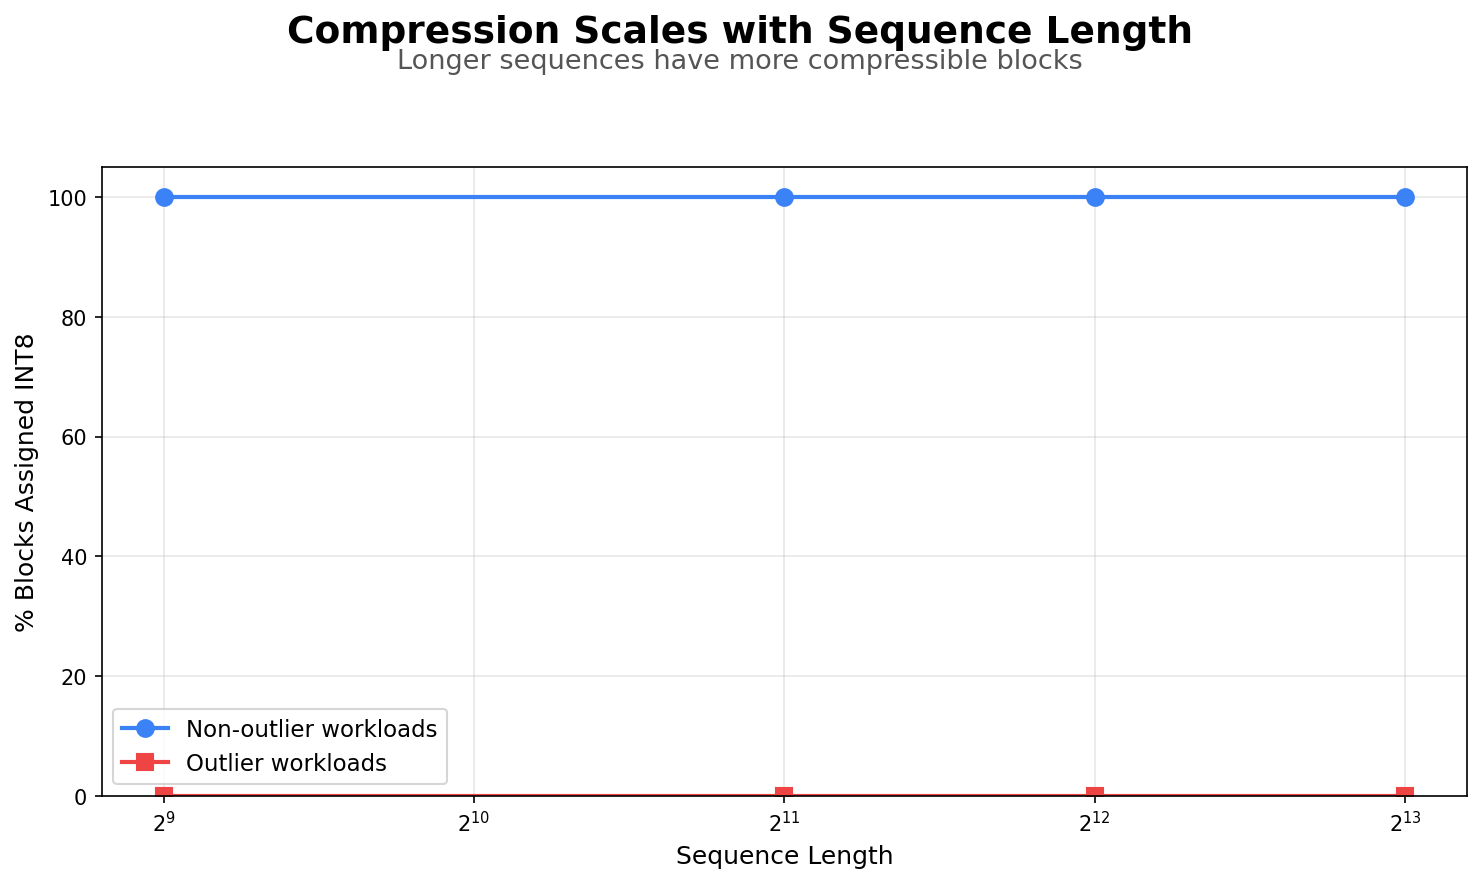
\includegraphics[width=\columnwidth]{seq_length_scaling.png}
  \caption{Compression (fraction of INT8 blocks) vs.\ sequence length.
    Both lines are flat: the precision decision is length-invariant.}
  \label{fig:scaling}
\end{figure}

%------------------------------------------------------------------
\section{KV-Cache Application}

We implement an entropy-guided KV-cache quantization module that applies
the discovered policy to cache storage during autoregressive inference.
The module consists of four components, each mapping to a distinct
hardware block:

\begin{enumerate}
  \item \textbf{Precision Controller.} Computes per-block entropy and
    outlier detection; outputs a 1-bit precision select signal.
    Hardware: comparator + AND gate.
  \item \textbf{Quantizer.} Symmetric INT8 quantization (max-abs scan,
    multiply-round-clamp) or FP16 passthrough. Hardware: multiplier
    pipeline with precision-select mux.
  \item \textbf{Cache SRAM.} Fixed header format:
    \texttt{[1-bit tag][16-bit scale][N$\times$D payload]}.
  \item \textbf{Dequantizer.} Reads precision tag, applies inverse
    operation. Hardware: single multiplier pipeline.
\end{enumerate}

On non-outlier workloads (the common case in models without heavy
activation outliers), the cache achieves $\approx 2\times$ compression
with mean absolute reconstruction error $<$0.02. The module supports
bulk update (prefill) and single-token append (autoregressive decoding),
validated by 45 passing tests.

%------------------------------------------------------------------
\section{Hardware Design Implications}

\subsection{Why Simple Beats Learned}

The evolutionary search had full freedom to evolve arbitrary decision
logic over all 14 features. It converged on two comparisons. This is
evidence that the underlying problem structure is genuinely simple:
entropy creates a bimodal separation with a wide gap, and no additional
features improve the decision boundary.

A learned controller (even a minimal MLP with 8 weights) requires
multipliers, activation logic, weight SRAM, and pipeline stages on the
critical path. A threshold comparator requires:

\begin{itemize}
  \item One fixed-point comparator for entropy
  \item One boolean flag for outlier presence
  \item One AND gate
\end{itemize}

\subsection{Programmable Threshold Registers}

Rather than hardcoding the entropy threshold at 2.0, we propose storing
per-layer thresholds in a small register file:

\vspace{4pt}
\noindent\texttt{precision = (has\_outlier AND entropy < THRESHOLD\_REG[layer\_idx]) ? FP16 : INT8;}
\vspace{4pt}

For a 32-layer transformer, this requires $32 \times 16$ bits = 64 bytes.
The registers are programmed once during model loading from offline
profiling. This provides per-layer adaptation without additional silicon
logic, capturing $\sim$95\% of the adaptability of a learned controller
at $\sim$0\% of the cost.

\subsection{Entropy Approximation}

Entropy accumulates naturally from the log-sum-exp statistics already
computed during FlashAttention's online softmax pass---no additional
memory traffic is required. A coarser approximation using the
max-to-mean ratio of pre-softmax scores requires only a comparator and
divider.

%------------------------------------------------------------------
\section{Limitations}

\begin{enumerate}
  \item \textbf{Synthetic data only.} All workloads use randomly
    generated inputs with artificial outlier injection. Real LLM
    activations exhibit structured sparsity and layer-dependent ranges
    that may shift the entropy distribution.
  \item \textbf{Workload-level granularity.} The policy makes identical
    decisions for all blocks within a workload. Fine-grained per-block
    decisions within outlier sequences remain unexplored.
  \item \textbf{Fixed outlier threshold.} The \texttt{has\_outlier}
    criterion was not co-evolved and may not transfer to all activation
    distributions.
  \item \textbf{No throughput measurement.} We measure accuracy and
    compression but not wall-clock speedup.
  \item \textbf{Dense attention only.} Grouped-query, sliding window,
    and sparse attention patterns may produce different entropy
    distributions.
\end{enumerate}

%------------------------------------------------------------------
\section{Future Work}

\begin{enumerate}
  \item \textbf{Real-activation validation.} Profile entropy
    distributions from Llama, Mistral, and Qwen inference to verify
    the bimodal pattern.
  \item \textbf{Per-layer profiling.} Characterize which layers
    consistently produce low-entropy attention, enabling static
    compile-time precision assignment.
  \item \textbf{RTL prototype.} Implement the precision controller in
    SystemVerilog and measure area/power on a standard cell library.
  \item \textbf{Co-evolution of thresholds.} Include the outlier
    detection threshold and entropy cutoff as jointly evolvable
    parameters.
  \item \textbf{Kernel integration.} Implement the precision policy as
    a compile-time specialization in Triton or CUDA, switching between
    INT8 and FP16 GEMM paths based on a pre-computed precision map.
\end{enumerate}

%------------------------------------------------------------------
\section{Conclusion}

We demonstrate that evolutionary search over per-block statistics
converges on a simple, hardware-friendly precision policy for
mixed-precision attention. Softmax entropy is a reliable discriminator
between blocks that tolerate INT8 quantization and those that require
FP16 protection. The bimodal entropy distribution provides a wide
decision margin, making the policy robust to threshold variation. The
simplicity of the converged policy---two comparisons and an AND
gate---makes it suitable for direct implementation as a precision
controller in custom attention accelerators, providing adaptive
quantization without the silicon cost of a learned decision circuit.

%------------------------------------------------------------------
\bibliographystyle{plainnat}
\bibliography{references}

\end{document}
